\documentclass[11pt,A4Paper]{article}
\usepackage[utf8]{inputenc}
\usepackage[a4paper,margin=1.5cm,top=2cm]{geometry}
\usepackage{graphicx}
\graphicspath{/Users/JohnnyLin/Desktop/Dzmitry_Lab /UROPS/uropsReport/figures}
\usepackage{float}
\usepackage{gensymb}
\usepackage{datetime}
\setlength{\parindent}{0pt}
\usepackage{appendix}
\usepackage{amsmath}
\usepackage[stable]{footmisc} %for footnote in title
\usepackage[hidelinks]{hyperref}
\usepackage{multirow,multicol}
\usepackage{adjustbox}
\usepackage{fancyhdr}
\usepackage{parskip}
\pagestyle{fancy}
% \fancyhf{}
\rhead{UROPS-CQT}
\lhead{Lin Zhonglin A0222183N}

\title{UROPS Report}
\author{Lin Zhonglin \hspace{1cm} A0222183N}
\usdate{}

\begin{document}
\maketitle

\section{Introduction}


\section{Background}
\begin{enumerate}
    \item introduction of our lab -> refer to the trapped Ytterbium ion paper
    \item what did I do
    \item how do the stuff I did relate to the lab in general
\end{enumerate}

\section{Building and tuning 638nm Grating Stabilized Compact Laser}
\subsection{Theory}
\begin{enumerate}
    \item lasers in general
    \item diode laser + reference that compact laser paper
    \item Gaussian beam optics
    \item geometric optics -> different lens system 
\end{enumerate}

\subsubsection{Gaussian optics}
different modes of a laser + relate to mode hopping in "Tuning laser" section

..\subsection{Building and Tuning The Laser}
\cite{compactGratingDiodeLaser}theory about tuning a diode laser: frequency jumping + how I adjusted temp, current, angle of grating to tune frequency + discuss how the process can be automated.
temp: don't let temp go below due point (about 17) 

\begin{figure}[H]
    \centering
    \includegraphics[width=0.5\textwidth]{638laser.HEIC}
    \caption{638nm laser}
    \label{fig:638laser}
\end{figure}

\subsection{Fiber Coupling}
(Coupling laser into a single-mode optical fiber) 
brief theory + detailed steps of it being done + how can be done better (automation) 
% 2. Coupling a beam into a fibre 
%     1. 用laser pen
%     2. 在两个位置,分别用两个自由度调
%     3. 最后提高功率,取出激光笔,四个扭左右转一转直到有光从fiber出来
    
1. Using a power meter 
    1. Adjust the 4 knobs independently → find the maximum point for each knob
    2. Walking the beam (horizontal and vertical → do separately)
        1. defining one mirror and trying to compensate with the other mirror 
            1. if cannot compensate, the detuned mirror is turned in the wrong direction
            2. Else try until maximum combination found

About local maxima: 

1. In the initial stage: scan through a larger range to find the global maxima among the many local maxima 
2. Later state: constantly check for whether the maxima being optimised is a local maximum → by turning left and right a bit more

# Cleaning Fibre

- Possible reasons for the fibre being dirty:
    - Dirt attached due to electrostatic attraction
- Draw out a new section of cloth
- Draw figure 8 multiple times until clean
- Look at the fibre using both side lighting and perpendicular lighting
- Spray acetone onto cloth and continue with figure 8 movement
    - Maybe debris on fibre is soluble

sources: 
1. https://www.researchgate.net/post/How-to-couple-laser-light-into-a-single-mode-fiber
2. https://www.youtube.com/watch?v=kQvhbJbDG0M


\subsection{Beam Characterisation}
\begin{enumerate}
    \item knife edge measurement (rational, procedure, put up some photos)
    \item photo diode (attach code in annex)
    \item can compare the two methods
    \item fitting measurement data with gaussian approx to recover gaussian beam parameters 
    \item possibility of automating the process
    \item beam shaping: anamorphic prisms / lens
\end{enumerate}

\subsubsection{Beam Collimation}
brief literature review + what I did + what it can be done better if higher precision is needed
\begin{enumerate}
    \item using a iris for horizontal and vertical alignment
    \item measure the umerical aperture of the fiber + tuning a fiber mount lens for collimation + finding the gaussian parameters again thorugh beam spot characterisation and back-fitting
\end{enumerate}




\subsection{Section conclusion}
what is this particular 638nm used in the lab for? -> for switching the trapped ion's state right? 


\section{Building and tuning Reference Cavity for 935nm laser}
\subsection{Theory}
theory about Fabry–Pérot cavity + relevant paper 




\subsection{Optical cavity allignment and coupling}
detailed steps + photos of apparatus + possble steps for better alignment

mode matching -> see notion for detail

\subsection{Sideband Checking}
discuss how can the cavity be used for this + detailed description of setup + pictures (if have time)



\subsection{Wavelength Measurement}
figure out how to use it to measure wavelength


\section{EOM (Electro-optic Modulator)}
% put basic intro to an EOM here 
In certain types of crystals it is possible to effect a change in the index of refraction that is proportional to the applied electric field. This is the linear electro-opic effect (also known as the Pockels effect). Applying a modulated electric field across such a nonlinear crystal (usualy the KDP type) and passing a beam of laser through the crystal leads to the laser beam being modulated in phase. (detail see: \cite{fundamentalsOfPhotonics}

\subsection{Theory and Model}
When a time-varying electric field is applied to the nonlinear crystal inside the EOM, the index of refraction $n$ changes in a sinusoidal manner resulting in phase modulation of the laser beam passing through the crystal. Consider the following short mathematical example to see that phase modulation is equivalent to frequency: 
\\
% 见激光原理for this part
Suppose instantaneous electric field at a point of EM wave of a laser beam: 
\begin{align*}
    E_c(t) = A_c cos(\omega_c T + \varphi_c)
\end{align*}
With phase modulation (assume sinusoidal modulation), we have final phase of the electric field of the EM wave: 
\begin{align*}
    \psi(t) &= \omega_c t + \varphi_c + \Delta \varphi (t) \\
            &= \omega_c t + \varphi_c + m_{\varphi} sin(\omega_m t)
\end{align*}
So the modulated electric field now becomes: 
\begin{align}
    E(t) &= A_c cos[ \omega_c t + m_{\varphi} sin(\omega_m t) + \varphi_c] \label{eqn:7.1.9}\\
         &= A_c cos\left\{  \int_0^t [ \omega_c + \Delta ]\omega(t)] dt + \varphi_c \right\} \\
\end{align}
where, 
\begin{equation*}
    \Delta \omega (t) = \frac{d\Delta \varphi (t)}{dt}
\end{equation*}
If we do Fourier transform to Eqn \ref{eqn:7.1.9}, we obtain in frequency space: 
\begin{equation}
    E(\omega) = A_c J_0(m) \delta(\omega - \omega_c) + A_c\sum_{n=1}^\infty J_m(m) \left\{ \delta[\omega-(\omega_c + n\omega_m)] +(-1)^n\delta[\omega-(\omega_c-n\omega_m)]\right\}
    \label{eqn:7.1.10}
\end{equation}

Eqn \ref{eqn:7.1.10} shows that when a single-frequency laser beam is modulated by a sinusoidal frequency, the modulated beam in frequency space comprises of the unmodulated frequency $\omega_0$ and infinite sidebands. Sideband frequency spacing is $\omega_m$, modulation frequency. 
% actually not sure about this, need to double check the math
Sideband amplitudes are determined by the Bessel function $J_n(m)$. (See Fig \ref{fig:EOMsidebandTheory}) What's of concern in this case is that EOM phase modulation produces frequency sidebands of laser beam. 

\begin{figure}[H]
    \centering
    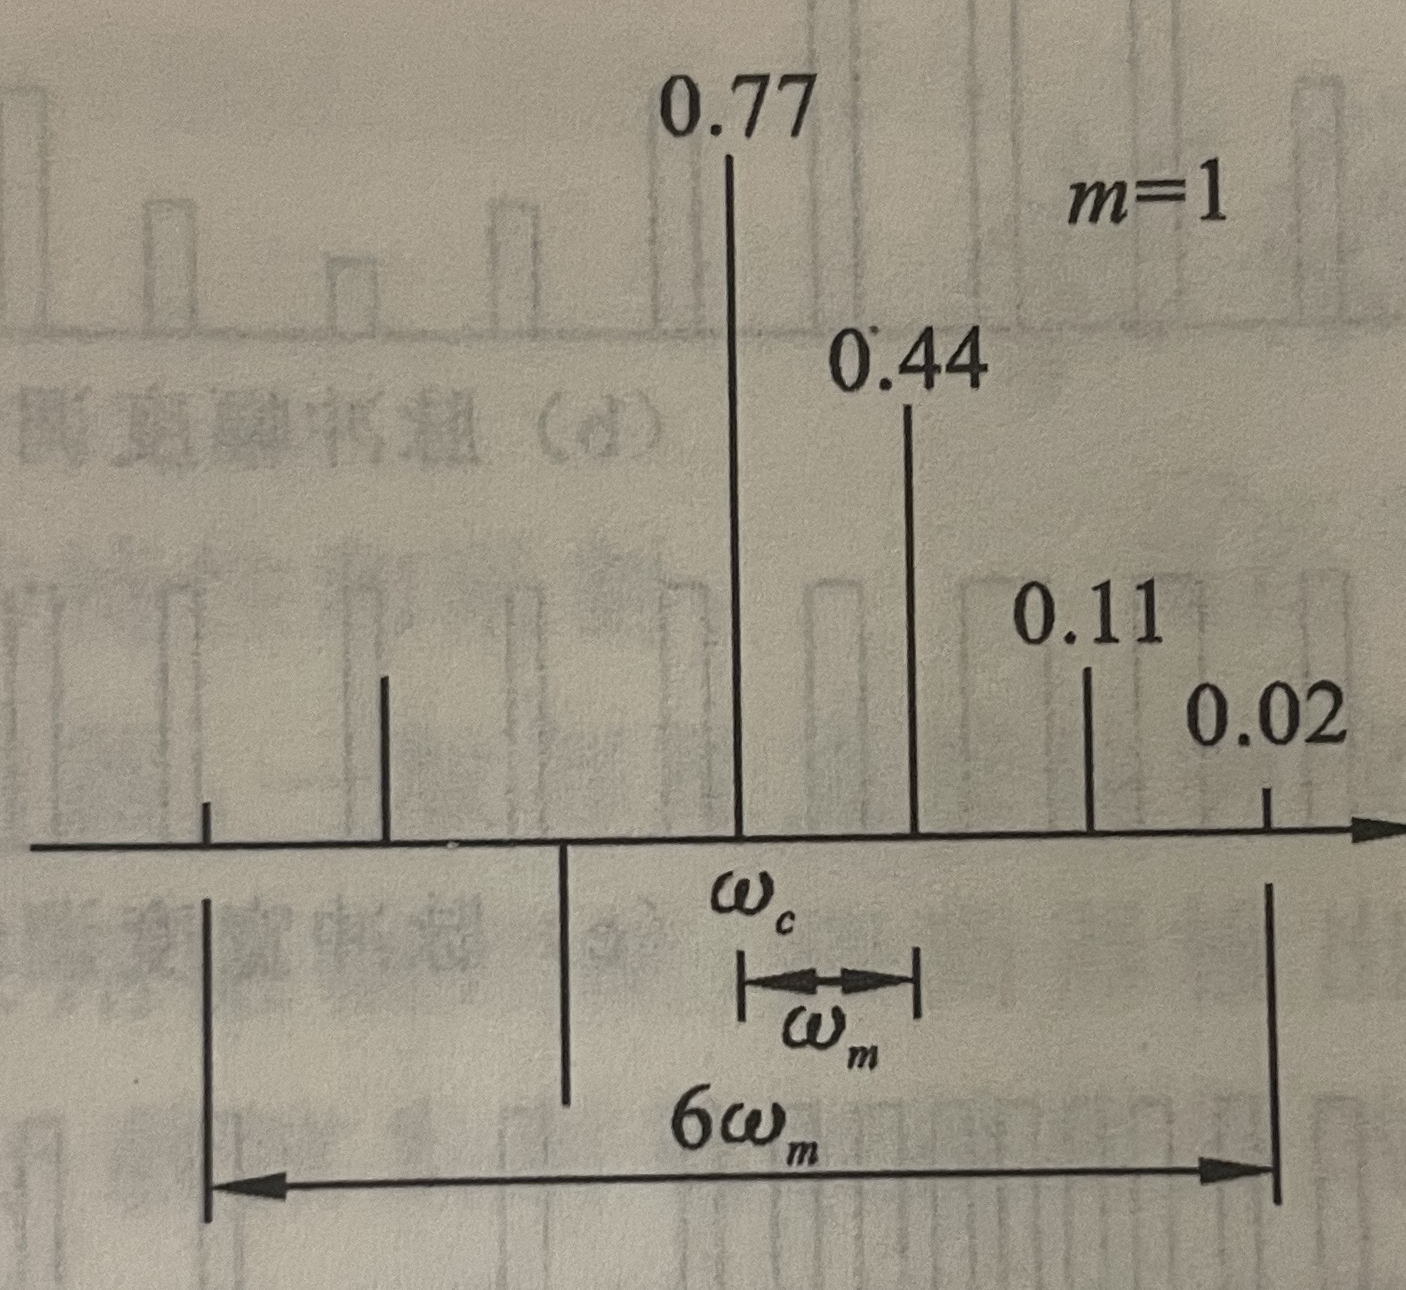
\includegraphics[width=0.3\textwidth]{EOMsidebandTheory.png}
    \caption{modulated laser beam frequency sepctrum}
    \label{fig:EOMsidebandTheory}
\end{figure}

 \subsection{EOM Tank Circuit Board: Model and Construction}
To construct an EOM tank circuit board and tune it to a partiular frequency, the following sources are useful: 
\begin{enumerate}
    \item paper: Design and construction of an efficient electro-optic modulator for laser spectroscopy\cite{20MHzEOM}
    \item textbook: Fundamentals of Photonics\cite{fundamentalsOfPhotonics}
    \item Prof Christian group's internal wiki has an entry on "How to build an EOM". There is a set of detailed note on EOM construction written by Meng Khoon. 
\end{enumerate}
The schematic of EOM circuit board is shown in Fig \ref{fig:eom-tank-cirucuit1}. Note that the components L, $C_1$, $C_2$ are nonideal components, i.e. the parasitics are ignored here.
$C_1$ refers to EOM crystal (ideally with correct AR coating for the relevant wavelength, in my case $\approx$738nm and $\approx$965nm)

\begin{figure}[H]
    \centering
    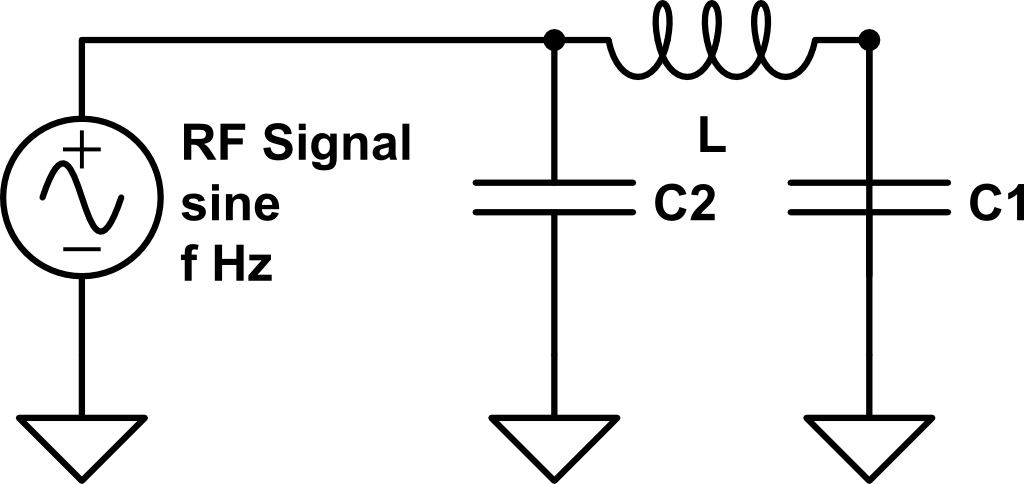
\includegraphics[width=.5\textwidth]{eom-tank-cirucuit1.png}
    \caption{EOM tank circuit board schematic (non-ideal component)}
    \label{fig:eom-tank-cirucuit1}
\end{figure}

The task of constructing an EOM at a particular modulation frequency can be be roughly be broken into the following three steps:
\par
Firstly, the LC circuit is in place to act as an amplifier so that the EOM can driven with low-power RF source of $<$ 1W, yet still providing significant electric field across the crystal for phase modulation. 
\par
Since we have an intended EOM modulation frequency frequency $f_0$, and the capacitance of the EOM crystal $C_1$ is fixed, we need to measure $C_2$ in order to backcalculate the inductor $L$ needed. Since the capacitor is small at the $pF$ level, we need to characterise $C_1$ by hooking it up with a suitable resistor, sending a square wave through it and determine its response time. Although the capacitance of the crystal should be predominantly determined by the crystal dielectric, my observation showed that the way that it's glued to the tank circuit also affects. I used silver containing glue spreaded evenly under the crystal and attached the crystal to the EOM tank circuit board's exposed copper section. The conductive glue is such that bottom of the crystal has a common ground hence electric field across the crystal will be near homogeneous as wanted. For my crystal with the way that it was glued, $C_1 \approx 3 \micro F$.
%TODO: insert measurements of crystal capacitance here
\par
After measurement of $C_1$, we can estimate the capacitance of the tank circuit board to be $C' = \frac{C_1C_2}{C_1+C_2} \approx C_1$. This is because $C_1 \gg C_2$ where $C_2$ is a coupling capacitor that will be explained later. The resonant frequency of the tank circuit can be estimated to be $f = \frac{\omega}{2\pi} = \frac{1}{2\pi\sqrt{LC'^2}}$. Rearranging to get $L = \frac{1}{(2\pi f C_1)^2}$, to get a resonant frequency of about 35 MHz, a $2 \micro H$ inductor is needed, the closest off-the-shelf inductor is $2.2 \micro H$. 
\par
Next the overall impedance of the EOM tank circuit needs to be matched to be $50\ohm$ such such that RF signal going to the EOM tank will be mostly absorbed and not reflected. In order tune the overall impedance of the EOM tank circuit, a coupling capacitor $C_2$ is added as shown in schematic \ref{fig:eom-tank-cirucuit1}. The overall loss of the EOM tank circuit can be modelled by a resistor $R_p$ as shown in Fig \ref{fig:eom-tank-cirucuit2}. Here we consider the components ideal. Note that parasitic resistance can be dependent on signal frequency, environment and many others. Here take it as $ R_p \approx 15 \Ohm$ based on Meng Khoon's note. However, much more careful characterisations of the circuit can be done. The coupling capacitor does not affect the tank circuit resonant frequency significantly as $C_1 \gg C_2$. so $C' = \frac{C_1C_2}{C_1+C_2} \approx C_1$ as mentioned earlier.  

\begin{figure}[H]
    \centering
    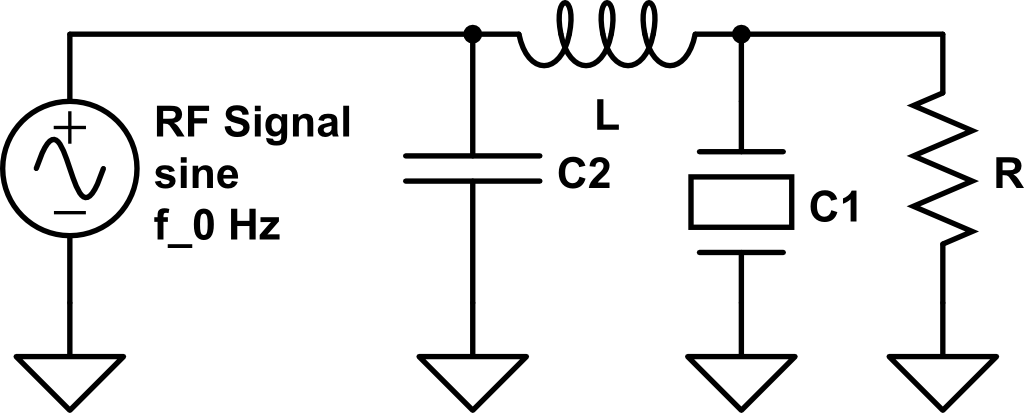
\includegraphics[width=.8\textwidth]{eom-tank-cirucuit2.png}
    \caption{EOM tank circuit, modelling overall loss}
    \label{fig:eom-tank-cirucuit2}
\end{figure}

We can calculate the overall impedance of the circuit based on this model. Setting overall impedance to be $50\Ohm$, the needed $C_2$ can be backcalculated to be $C_2 = \frac{\sqrt{50/R_p -1}}{50} \approx 93.8 nF$ which is indeed much smaller than $C_1 \approx 3 \micro F$. Choose a variable capacitor around this range of capacitance. 
\par
Lastly set up a measurement circuit as shown in Fig \ref{fig:eom-freq-measurement-setup.png}. Tune the variable capacitor until reflected signal from the EOM tank circuit board is minimum. Note that most variable capacitor has a tuning range of less than $360\degree$, so tune slowly until the valley shown on the spectrum analyser is the deepest. 

\begin{figure}[H]
    \centering
    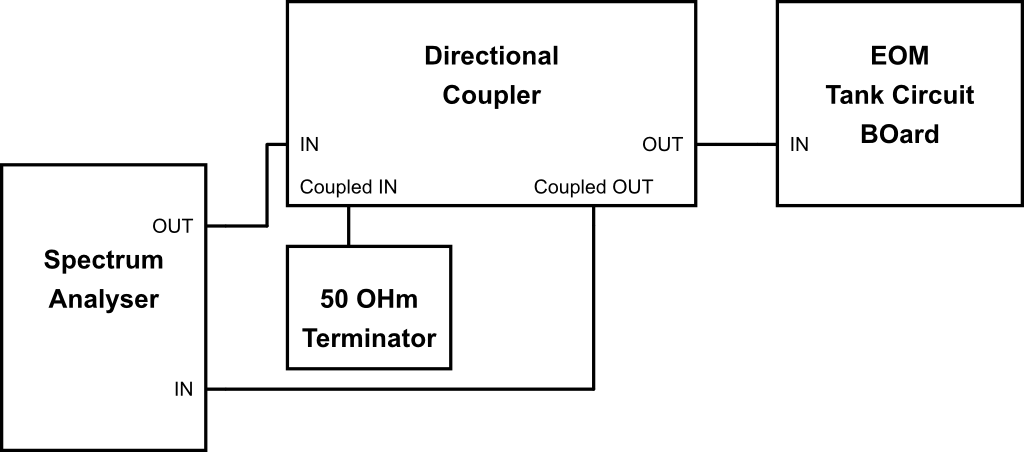
\includegraphics[width=0.8\textwidth]{eom-freq-measurement-setup.png}
    \caption{EOM frequency measurement setup}
    \label{fig:eom-freq-measurement-setup.png}
\end{figure}

After tuning the variable capacitor, my EOM tank circuit board has a resonant frequency $f_0 \approx 38 MHz$, see Fig \ref{fig:EOMfrequencyMeasurement}. 

\begin{figure}[H]
    \centering
    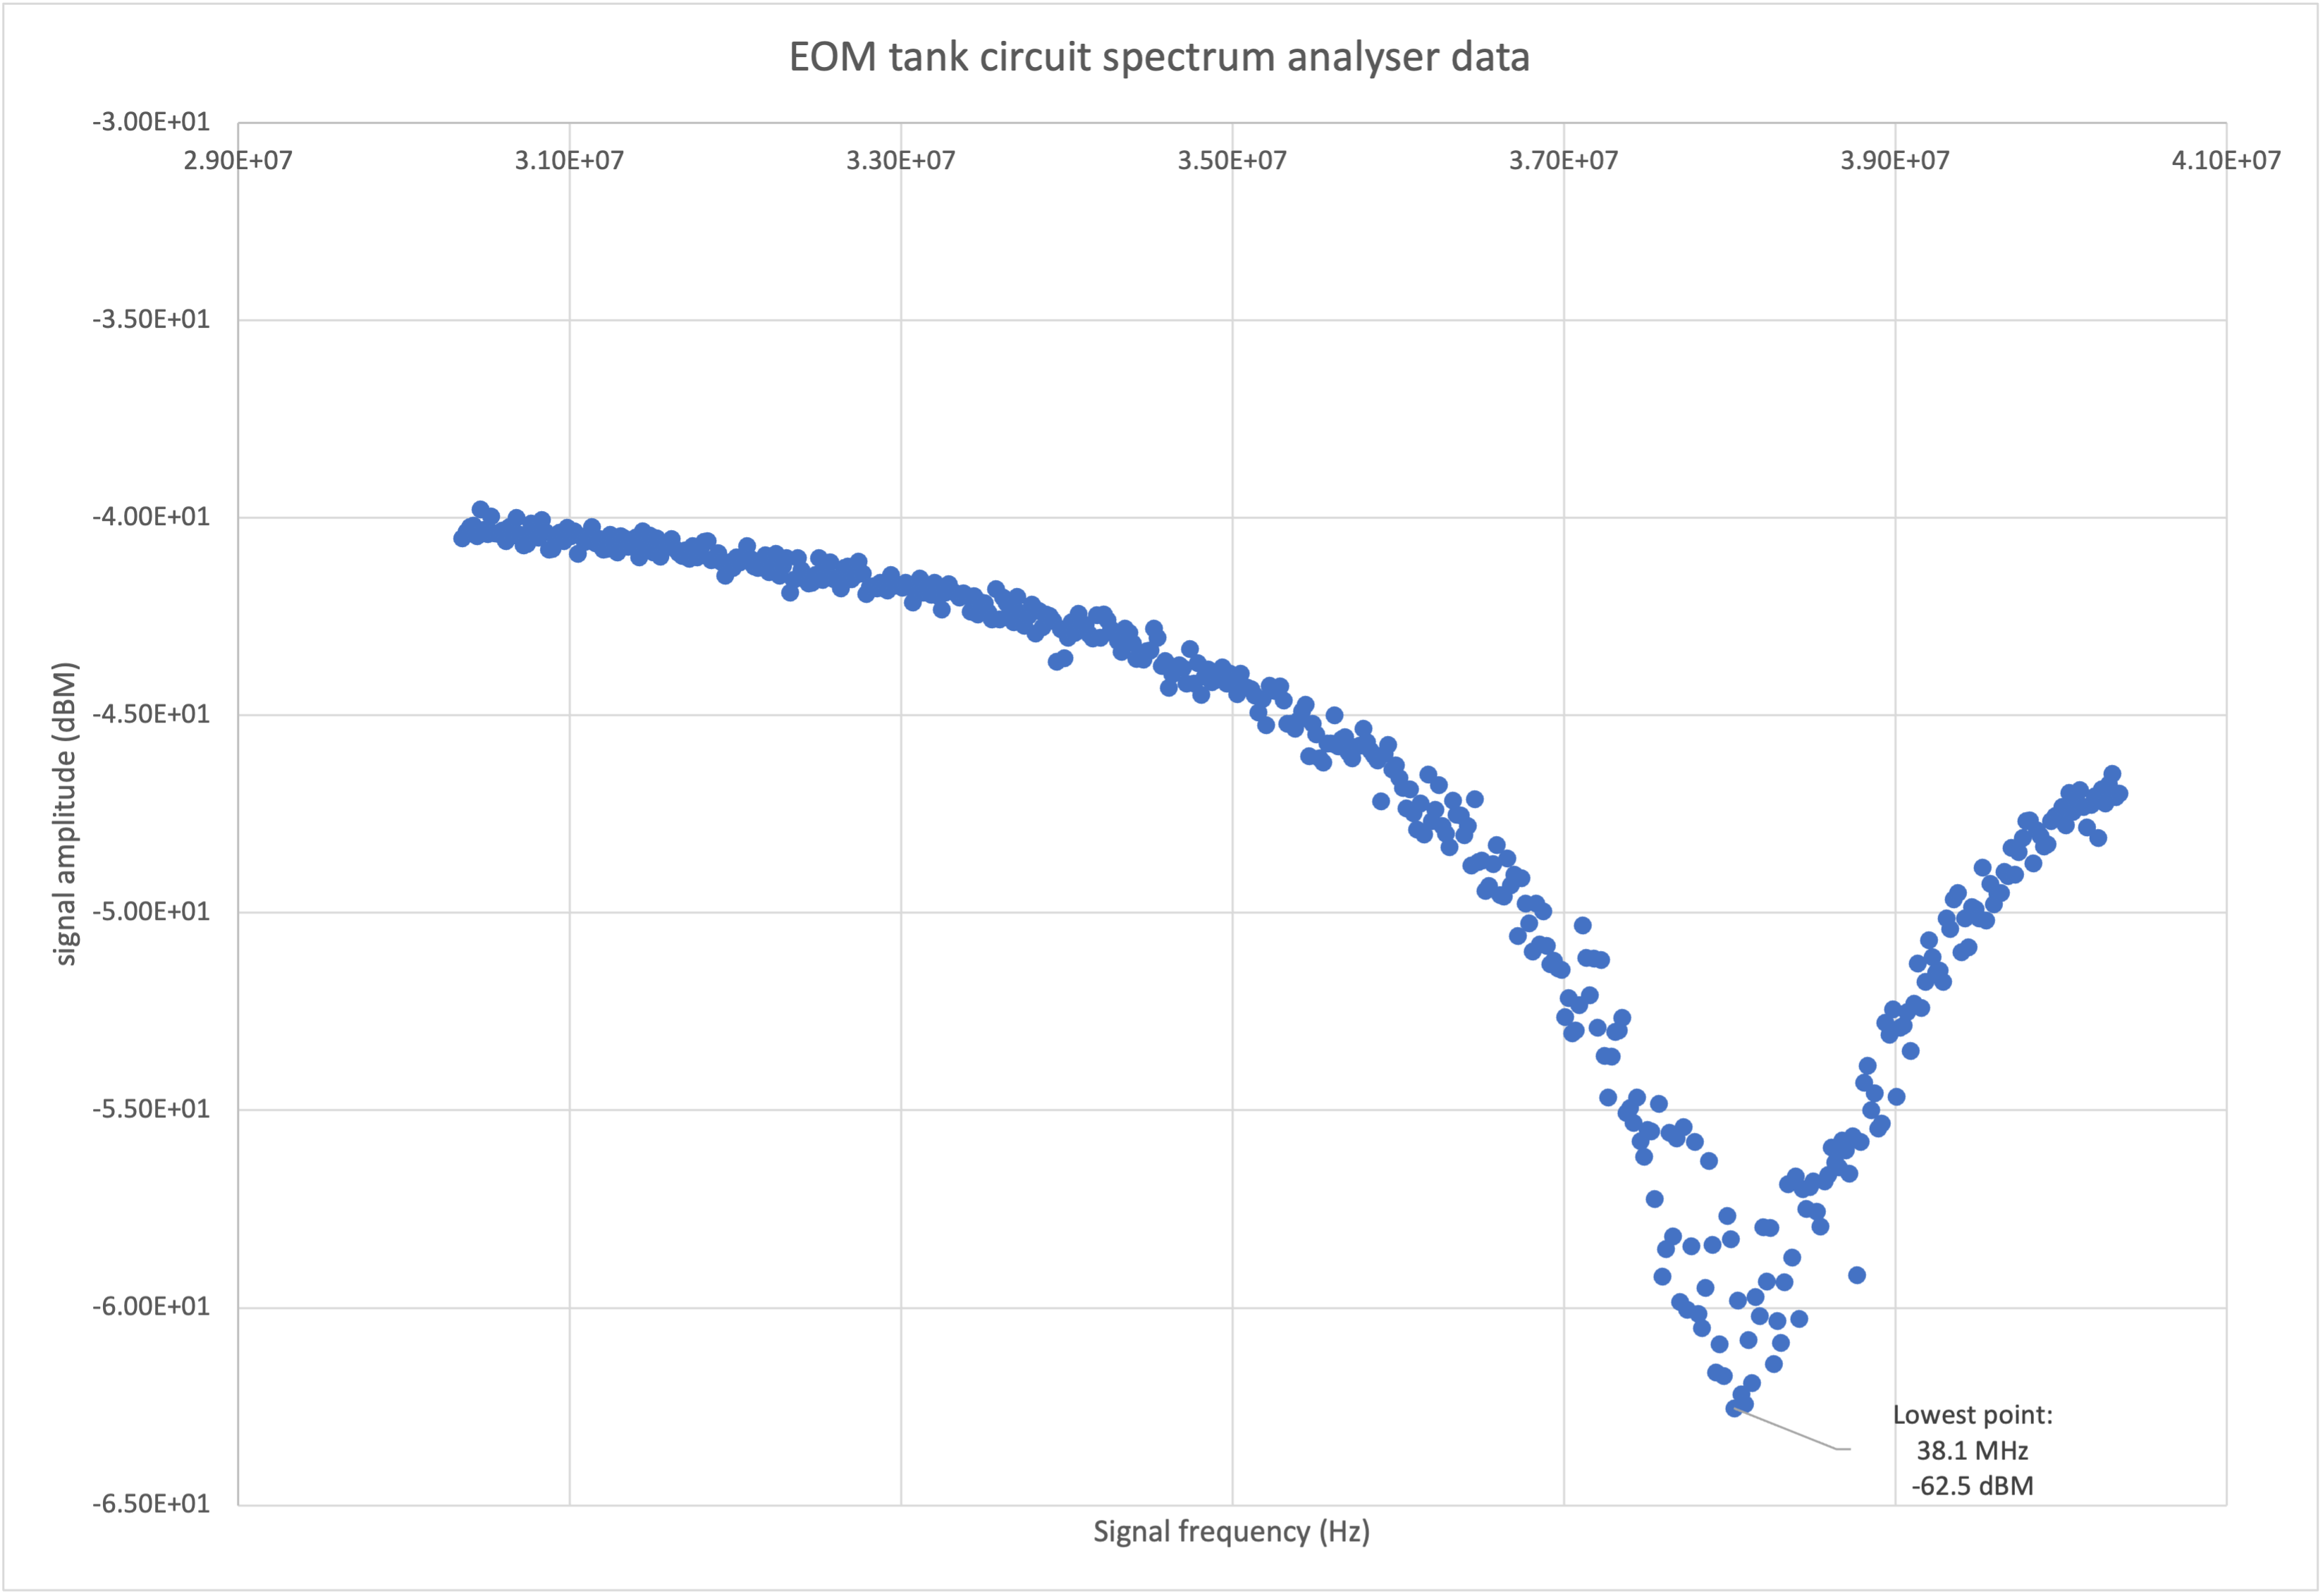
\includegraphics[width=0.8\textwidth]{EOMfrequencyMeasurement.png}
    \caption{EOM tank circuit frequency measurement setup}
    \label{fig:EOMfrequencyMeasurement}
\end{figure}

A final word on EOM construction: To improve on the Q-factor of the EOM tank circuit, parasitics of the circuit need to be better charactersied and subsequently matching impedance better. A better impedance matching will lead to higher efficiency of absorption of input RF signal. A small-voltage RF signal can bring about more significant modulation. However, my EOM as it currently is suffices for my subsequent task. 
%TODO: measure Q-factor of my EOM board
%TODO: insert an image of my actual EOM board here

\section{Fabry-Perot Cavity}
Laser resonators are open structures containing two or more mirrors that are aligned to produce optical feedback to the gain element. In the simplest case, a resonator consists of two aligned mirrors. These mirrors are called end mirrors and define the optical cavity. Optical radiation circulates within the cavity, bouncing back and forth between the end mirrors and passing through the gain element. An optical resonator can be characterised by the following parameters: 
\begin{enumerate}
    \item number of mirrors constituting the resonator
    \item focal length of mirrors
    \item radius of mirrors (usually small relative to cavity length)
    \item length of cavity
    \item reflectivity of mirrors
    \item other optical losses: how good is the vacuum in the cavity and so on
\end{enumerate}
What's relevant to this report is a particular type of optical resonator: confocal Fabry-Perot cavity. Fabry-Perot cavities are optical cavities with two parallel mirrors. Confocal Fabry-Perot cavities have focal points of the two concave mirrors overlapping at the center of the cavity as shown in Fig \ref{fig:confocalCavity}. The confocal cavity I used in experiment has a cavity length of L=15cm. 

\begin{figure}[H]
    \centering
    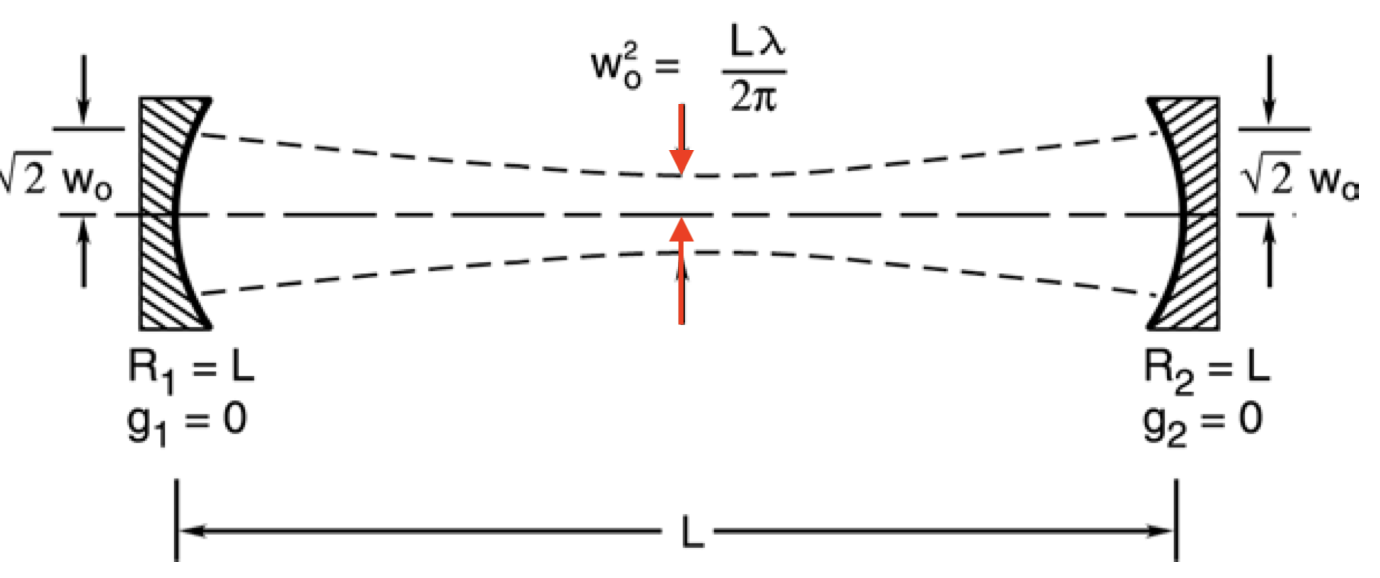
\includegraphics[width = .8\textwidth]{confocalCavity.png}
    \caption{Confocal cavity}
    \label{fig:confocalCavity}
\end{figure}

One good way to measure the frequency of a laser's beam is send it into a Fabry-Perot cavity and look at what gets transmitted (or reflected). Light can only pass through a Fabry-Perot cavity if twice the length of the cavity is equal to an integer number of wavelengths of the light. Or equivalently put, the frequency of the light's electromagnetic wave must be an integer number times the cavity's free spectral range $\Delta \nu_{fsr} \equiv c/2L$, where $L$ is the length of the cavity and $c$ is the speed of light. For my case $\Delta \nu_{fsr} \approx 1GHz$. The cavity acts as a filter, with transmission lines, or resonances, spaced evenly in frequency every free spectral range. Fig \ref{fig:cavityTransmission}  shows a plot of the fraction of light transmitted through a Fabry-Perot cavity versus the frequency of the light. \cite{PDHintro}\cite{fundamentalsOfPhotonics}

\begin{figure}[H]
    \centering
    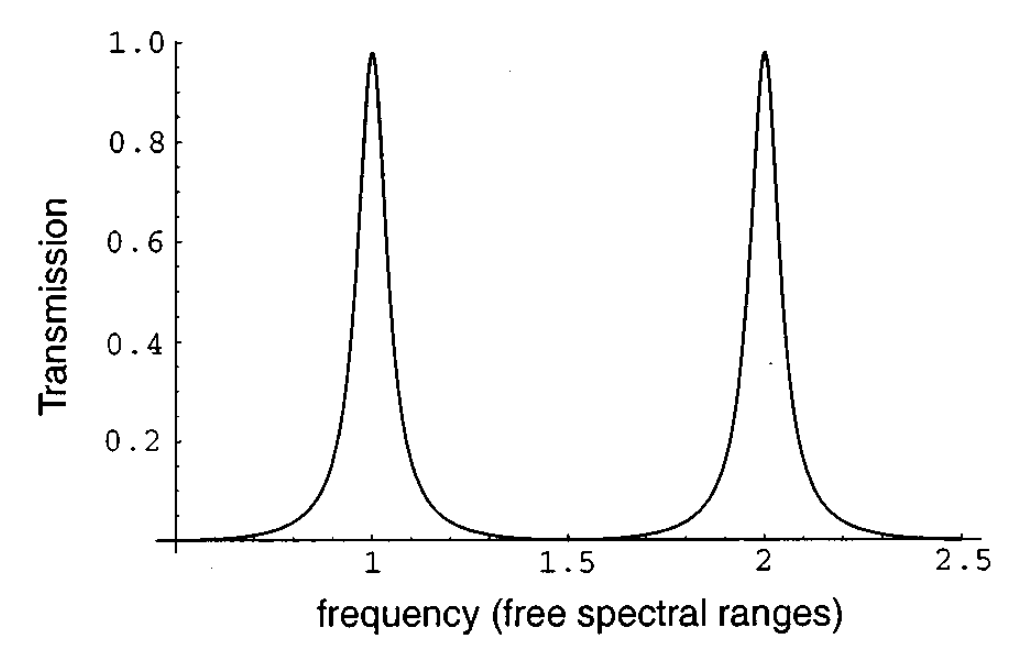
\includegraphics[width=.8\textwidth]{cavityTransmission.png}
    \caption{Cavity transmission}
    \label{fig:cavityTransmission}
\end{figure}

\subsection{Laser beam - Cavity Coupling}
To couple a well collimated laser beam with beam radius $\omega_1$ (see section on laser beam collimation and characterisation in this report) into a Fabry-Perot cavity, follow these steps: 
\begin{enumerate}
    \item Choose a thin lens (with relevant AR coating) of focal length $f$ to focus the laser beam from radius $\omega_1$ to $\omega_0$ at the center of the cavity. Gaussian beams have a propagating spherical wavefront, and each Gaussian beam is uniquely characterised by its beam waist, here being $\omega_0$. In the context of a confocal cavity, when a Gaussian has beam waist $\omega_0 = \frac{L\lambda}{2\pi}$ as shown in Fig \ref{fig:confocalCavity} the Gaussian beam spherical wavefront at the mirrors will match the curvatures of the mirrors, hence leading to stable standing waves to establish in the cavity. In my case, consider $L=15$ cm, $\lambda = 935.18848$ nm,  $\omega_0$ = $0.000149419$ m.
    
    \item To determine the focal length $f$, we consider how parameters of a Gaussian beam transforms through a thin convex lens (see \cite{principleOfLasersOrazio} for details). Approximately, we have $\omega' \approx \frac{\lambda f}{\pi \omega}$. Where, $\omega'$ is the 'image'-side beam waist, $\omega$ is the 'object'-side beam waist, $\lambda$ is laser beam wavelength, $f$ is the thin lens focal length. In my case, consider $\lambda = 935.18848$ nm, $\omega'$ = $0.000149419$ m. $\omega = 1.1$ mm (image-side beam radius is estimated to be so through beam characterisation) $f = frac{\omega' \pi \omega_1}{\lambda} \approx 0.552139m \approx 550mm$. However, using a lens of such focal length was not practical due to space constraint on the optical table, I used a $f=150mm$ thin lens as it was the longest focal length lens available off-the-shelf. 
    
    \item Pass the laser beam through at least one mirror before entering the cavity to obtain at least 2 points of adjustment. See Fig \ref{fig:laserCavityCoupling} in Appendix for a hand-written note on how to adjust the mirrors (or fibre mount) for optical coupling using a card (either normal paper or IR paper depending on wavelength) with a hole. 

    \item Lastly send a triangle wave signal of appropriate $V_{pp}$ to the piezo actuator to scan the cavity length across a certain range. The $V_{pp}$ needed depends on the scanning range needed and the behaviour of the piezo actuator. See chapter 2 of \cite{FundamentalPrinciplesofEngineeringNanometrology} for details on piezo actuators. For my case, after testing, a triangle wave generator board producing $\pm 5$V, together with a voltage gain board of coefficient 19 is used to produce a $V_{pp} \approx 190$V. 
\end{enumerate}

\section{Frequency Locking a Laser: Pound-Drever-Hall Method}
Following sources are relevant to the current section: 
\begin{enumerate}
    \item paper: An introduction to Pound–Drever–Hall laser frequency stabilization \cite{PDHintro}. This paper gives an overview of the scheme of Pound-Drever-Hall method. 
    \item paper: Laser phase and frequency stabilization using an optical resonator \cite{PDH1983}. This is original paper that proposed the PDH scheme in 1983. 
\end{enumerate}

Tunable lasers have multiple wavelength-selecting elements such as piezo-controlled etalons and gratings. Typically, the length of the lasing cavity is controlled by a voltage sent to a piezo-electric transducer. The laser-cavity length can change because of a number of factors such as temperature changes, and mechanical vibrations. These factors affect the laser-frequency stability. The standard PDH method of frequency-locking involves the following process: A laser's frequency is measured with a Fabry-Perot cavity, and this measurement is fed back to the laser to suppress\cite{PDH1983}\cite{PDHintro}.
\par
    
\begin{figure}[H]
    \centering
    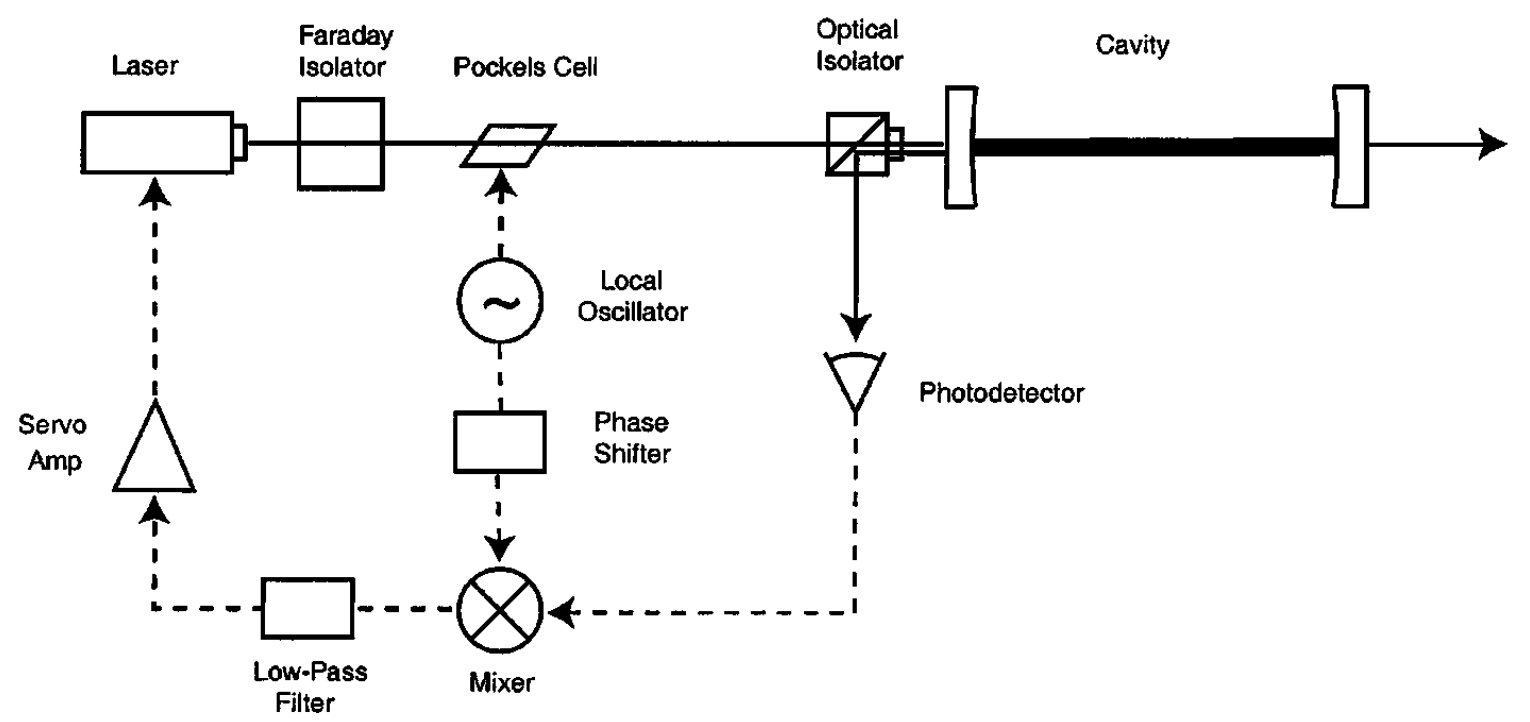
\includegraphics[width=.8\textwidth]{PDHlayout.png}
    \caption{The basic layout for locking a cavity to a laser. Solid lines are optical paths and dashed lines are signal paths. The signal going to the laser controls its frequency \cite{PDHintro}}
    \label{fig:PDHlayout}
\end{figure}

Referring to Fig \ref{fig:PDHlayout}, the basic steps of a PDH locking scheme is outlined as following: 
\begin{enumerate}
    \item 
    \item A laser beam is passed through a Pockels cell to modulate its frequency at a frequency small relative to the $\Delta \nu_{fsr}$ free spectral range of the optical cavity. My cavity has length $L=15$cm, $\Delta \nu_{fsr} = c/2L \approx 1GHz$. Hence my EOM at $\approx 38 MHz$, as discussed in the EOM section, is appropriate here. 
\end{enumerate}



\section{Other Discussions}
\subsection{General Optical Lab Techniques and devices}
\begin{enumerate}
    \item discuss various optical devices on the optical table (reference QDevice content): wave plates, polarisers, etc -> briefly on how they work + how to use them in the lab 
    \begin{enumerate}
        \item wave plates, polarisers
        \item AR coating
        \item laser power meter: wavelength selection -> response curve
        \item lens cleaning
        \item DIY relevant tools in the lab. exmaples: strips of paper for ray tracing
        \item electronics stuff: soldering, PCB board inspection
        
    \end{enumerate}
\end{enumerate}




\section{Conclusion}
\begin{enumerate}
    \item what have I learn: about theory and experimental physics lab
    \item what have I done 
    \item possible follow up investigations / improvement on existing current
\end{enumerate}

\section{Acknowledgements}
thank the lab people! Jaren, Muyoung, Dzmitry, Nigel, Kowei

\section{Appendix}
\begin{figure}[H]
    \centering
    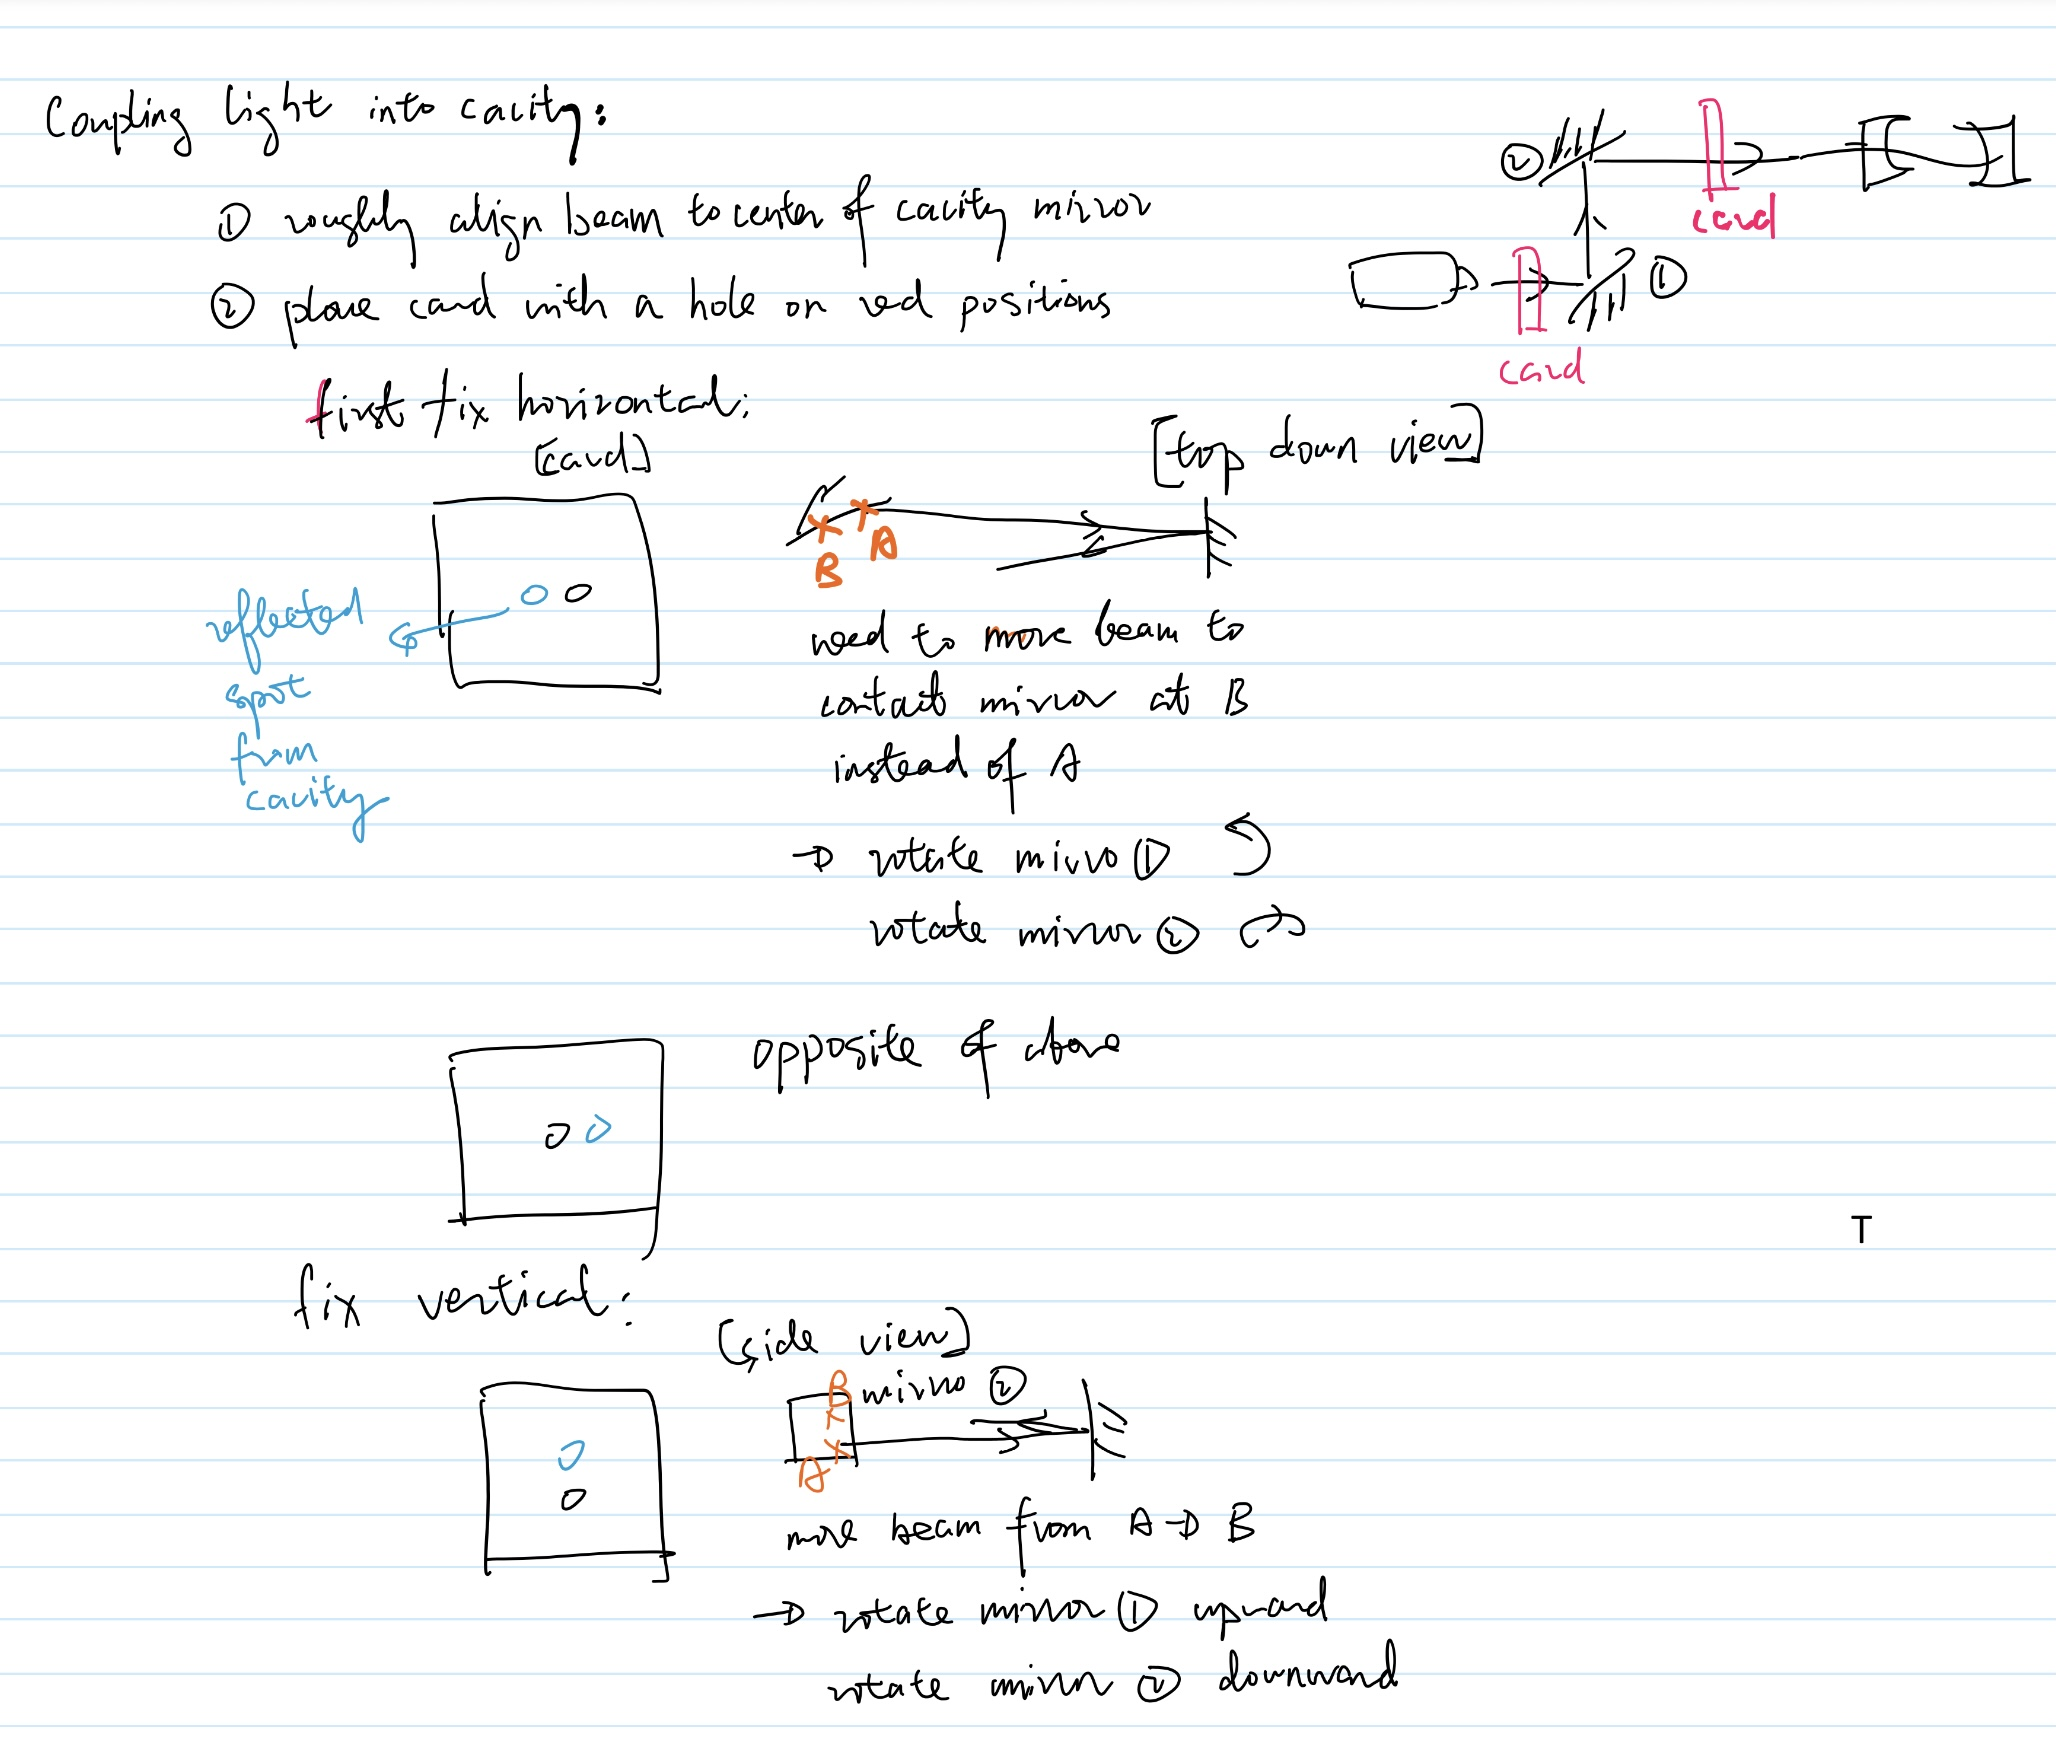
\includegraphics[width=\textwidth]{laserCavityCoupling.jpg}
    \caption{Laser beam - Cavity Coupling Note}
    \label{fig:laserCavityCoupling}
\end{figure}

\bibliographystyle{plain}
\bibliography{bibliography.bib}

\end{document}
